% questions.tex —— 2008 年·普通高等学校招生考试·北京卷·理科 · 题目内容片段（无答案）
% 由 tools/generate_projects.py 依来源总账自 2008/2008_数学真题_北京理_试题.md 生成，勿手改（改源 MD 后重跑）


状态：needs-review；依固定候选 PDF 两页（印刷页 425–426）三栏图像以 300 dpi 渲染逐题核验，图形已矢量重绘，正式构建与逐页验收待完成。源未列各题分值，不补分值。

\gkpart{一、选择题}

\begin{question}
\gkti{1}已知全集 $U=\mathbf R$，集合 $A=\{x\mid-2\leqslant x\leqslant3\}$，$B=\{x\mid x<-1\ \text{\text{或}}\ x>4\}$，那么集合 $A\cap(\complement_UB)$ 等于（　）

（A）$\{x\mid-2\leqslant x<4\}$

（B）$\{x\mid x\leqslant3\ \text{\text{或}}\ x\geqslant4\}$

（C）$\{x\mid-2\leqslant x<-1\}$

（D）$\{x\mid-1\leqslant x\leqslant3\}$

\end{question}
\begin{question}
\gkti{2}若 $a=2^{0.5}$，$b=\log_\pi3$，$c=\log_2\sin\dfrac{2\pi}5$，则（　）

（A）$a>b>c$

（B）$b>a>c$

（C）$c>a>b$

（D）$b>c>a$

\end{question}
\begin{question}
\gkti{3}“函数 $f(x)$（$x\in\mathbf R$）存在反函数”是“函数 $f(x)$ 在 $\mathbf R$ 上为增函数”的（　）

（A）充分而不必要条件

（B）必要而不充分条件

（C）充分必要条件

（D）既不充分也不必要条件

\end{question}
\begin{question}
\gkti{4}若点 $P$ 到直线 $x=-1$ 的距离比它到点 $(2,0)$ 的距离小 $1$，则点 $P$ 的轨迹为（　）

（A）圆

（B）椭圆

（C）双曲线

（D）抛物线

\end{question}
\begin{question}
\gkti{5}若实数 $x$，$y$ 满足 $\begin{cases}x-y+1\geqslant0,\\ x+y\geqslant0,\\ x\leqslant0,\end{cases}$ 则 $z=3^{x+2y}$ 的最小值是（　）

（A）$0$

（B）$1$

（C）$\sqrt3$

（D）$9$

\end{question}
\begin{question}
\gkti{6}已知数列 $\{a_n\}$ 对任意的 $p$，$q\in\mathbf N^*$ 满足 $a_{p+q}=a_p+a_q$，且 $a_2=-6$，那么 $a_{10}$ 等于（　）

（A）$-165$

（B）$-33$

（C）$-30$

（D）$-21$

\end{question}
\begingroup
\renewenvironment{question}{\Needspace{0.46\textheight}}{}
\begin{question}
\gkti{7}过直线 $y=x$ 上的一点作圆 $(x-5)^2+(y-1)^2=2$ 的两条切线 $l_1$，$l_2$，当直线 $l_1$，$l_2$ 关于 $y=x$ 对称时，它们之间的夹角为（　）

（A）$30^\circ$

（B）$45^\circ$

（C）$60^\circ$

（D）$90^\circ$

\Needspace{0.4\textheight}
\end{question}
\endgroup
\begin{question}
\gkti{8}如图，动点 $P$ 在正方体 $ABCD-A_1B_1C_1D_1$ 的对角线 $BD_1$ 上。过点 $P$ 作垂直于平面 $BB_1D_1D$ 的直线，与正方体表面相交于 $M$，$N$。设 $BP=x$，$MN=y$，则函数 $y=f(x)$ 的图象大致是（　）
\nopagebreak[4]
\begin{center}% 2008 年北京卷理科第 8 题：正方体 ABCD-A1B1C1D1，P 在体对角线 BD1 上，
%   过 P 作垂直于平面 BB1D1D 的直线，与正方体表面交于 M、N。
% 来源 PDF：gaokaomath-src/普通高考/2008/2008北京理.pdf
% SHA-256：1ba43840bfc822e6bcd4a1c04e69becd857890f1abf3da09910b4f26ae25c9a8
% 原页：2008北京理.pdf 第 1 页（A3 三栏）第 1 栏，书页码 425。
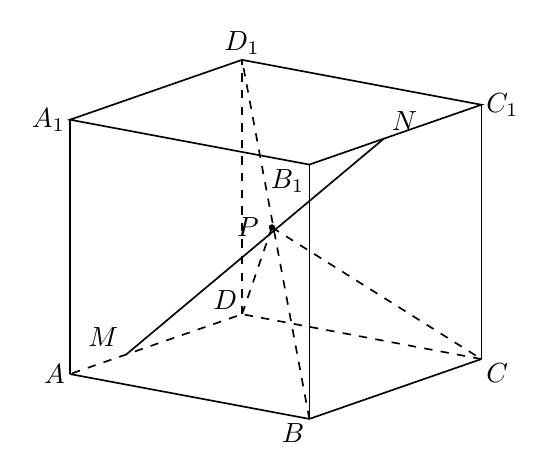
\begin{tikzpicture}[scale=0.95, semithick,
  every node/.style={inner sep=1.5pt}]
  \coordinate (A) at (0.0,0.9);
  \coordinate (B) at (3.2,0.3);
  \coordinate (C) at (5.5,1.1);
  \coordinate (D) at (2.3,1.7);
  \coordinate (A1) at (0.0,4.3);
  \coordinate (B1) at (3.2,3.7);
  \coordinate (C1) at (5.5,4.5);
  \coordinate (D1) at (2.3,5.1);

  \draw (A) -- (B) -- (C);
  \draw[dashed] (C) -- (D) -- (A);
  \draw (A) -- (A1);
  \draw (B) -- (B1);
  \draw (C) -- (C1);
  \draw (A1) -- (B1) -- (C1) -- (D1) -- cycle;
  \draw[dashed] (D) -- (D1);
  \draw[dashed] (B) -- (D1);

  % P 与过 P 的 MN（平行 AC）
  \coordinate (P) at (2.7,2.86);
  \coordinate (M) at (0.75,1.16);
  \coordinate (N) at (4.2,4.05);
  \draw (M) -- (N);
  \fill (P) circle (1.2pt);
  \draw[dashed] (P) -- (D);
  \draw[dashed] (P) -- (C);

  \node[left] at (A) {$A$};
  \node[below left] at (B) {$B$};
  \node[below right] at (C) {$C$};
  \node[above left] at (D) {$D$};
  \node[left] at (A1) {$A_1$};
  \node[below left] at (B1) {$B_1$};
  \node[right] at (C1) {$C_1$};
  \node[above] at (D1) {$D_1$};
  \node[left=3pt] at (P) {$P$};
  \node[above left=1pt] at (M) {$M$};
  \node[above right=1pt] at (N) {$N$};
\end{tikzpicture}
\end{center}
\nopagebreak[4]
四种候选图象如下：
\nopagebreak[4]
\begin{center}% 2008 年北京卷理科第 8 题的四个候选图象：(A) 梯形、(B) 三角形、(C) 不对称梯形、(D) 钟形曲线。
% 来源 PDF、SHA-256 同 q8_cube。
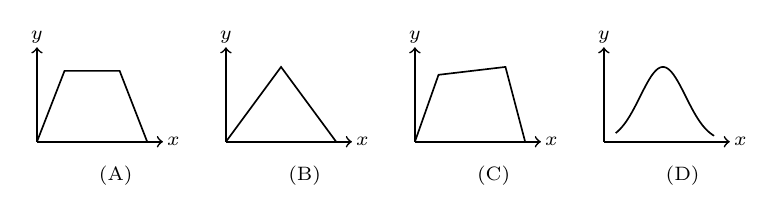
\begin{tikzpicture}[semithick, every node/.style={inner sep=1.2pt}]
  % (A)
  \begin{scope}[shift={(0,0)}]
    \draw[->] (0,0) -- (1.6,0) node[right,font=\scriptsize] {$x$};
    \draw[->] (0,0) -- (0,1.2) node[above,font=\scriptsize] {$y$};
    \draw (0,0) -- (0.35,0.9) -- (1.05,0.9) -- (1.4,0);
    \node[below,font=\scriptsize] at (1.0,-0.25) {(A)};
  \end{scope}
  % (B)
  \begin{scope}[shift={(2.4,0)}]
    \draw[->] (0,0) -- (1.6,0) node[right,font=\scriptsize] {$x$};
    \draw[->] (0,0) -- (0,1.2) node[above,font=\scriptsize] {$y$};
    \draw (0,0) -- (0.7,0.95) -- (1.4,0);
    \node[below,font=\scriptsize] at (1.0,-0.25) {(B)};
  \end{scope}
  % (C)
  \begin{scope}[shift={(4.8,0)}]
    \draw[->] (0,0) -- (1.6,0) node[right,font=\scriptsize] {$x$};
    \draw[->] (0,0) -- (0,1.2) node[above,font=\scriptsize] {$y$};
    \draw (0,0) -- (0.3,0.85) -- (1.15,0.95) -- (1.4,0);
    \node[below,font=\scriptsize] at (1.0,-0.25) {(C)};
  \end{scope}
  % (D)
  \begin{scope}[shift={(7.2,0)}]
    \draw[->] (0,0) -- (1.6,0) node[right,font=\scriptsize] {$x$};
    \draw[->] (0,0) -- (0,1.2) node[above,font=\scriptsize] {$y$};
    \draw[domain=0.15:1.4, samples=50] plot (\x,{0.95*exp(-6*(\x-0.75)*(\x-0.75))});
    \node[below,font=\scriptsize] at (1.0,-0.25) {(D)};
  \end{scope}
\end{tikzpicture}
\end{center}
\nopagebreak[4]
\end{question}
\gkpart{二、填空题}

\begin{question}
\gkti{9}已知 $(a-\mathrm i)^2=2\mathrm i$，其中 $\mathrm i$ 是虚数单位，那么实数 $a=$\gkblank{}。

\end{question}
\begin{question}
\gkti{10}已知向量 $\boldsymbol a$ 与 $\boldsymbol b$ 的夹角为 $120^\circ$，且 $|\boldsymbol a|=|\boldsymbol b|=4$，那么 $\boldsymbol b\cdot(2\boldsymbol a+\boldsymbol b)$ 的值为\gkblank{}。

\end{question}
\begingroup
\renewenvironment{question}{\Needspace{0.44\textheight}}{}
\begin{question}
\gkti{11}若 $\left(x^2+\dfrac1{x^3}\right)^n$ 展开式的各项系数之和为 $32$，则 $n=$\gkblank{}，其展开式中的常数项为\gkblank{}。（用数字作答）

\Needspace{0.4\textheight}
\end{question}
\endgroup
\begin{question}
\gkti{12}如图，函数 $f(x)$ 的图象是折线段 $ABC$，其中 $A$，$B$，$C$ 的坐标分别为 $(0,4)$，$(2,0)$，$(6,4)$，则 $f(f(0))=$\gkblank{}；$\lim\limits_{\Delta x\to0}\dfrac{f(1+\Delta x)-f(1)}{\Delta x}=$\gkblank{}。（用数字作答）
\nopagebreak[4]
\begin{center}% 2008 年北京卷理科第 12 题：折线 ABC，A(0,4)、B(2,0)、C(6,4)。
% 来源 PDF：gaokaomath-src/普通高考/2008/2008北京理.pdf
% SHA-256：1ba43840bfc822e6bcd4a1c04e69becd857890f1abf3da09910b4f26ae25c9a8
% 原页：2008北京理.pdf 第 1 页（A3 三栏）第 2 栏，书页码 425。
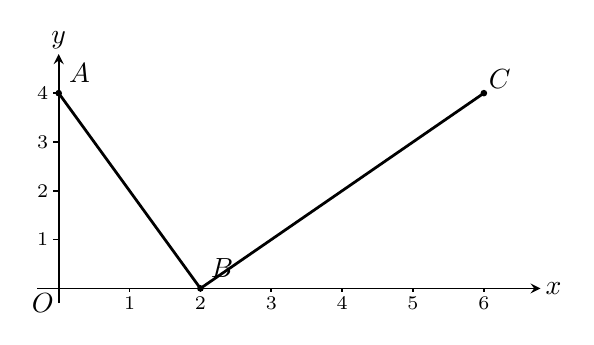
\begin{tikzpicture}[x=0.9cm, y=0.62cm, semithick,
  every node/.style={inner sep=1.5pt}]
  \draw[->,>=stealth] (-0.3,0) -- (6.8,0) node[right] {$x$};
  \draw[->,>=stealth] (0,-0.3) -- (0,4.8) node[above] {$y$};
  \node[below left] at (0,0) {$O$};
  \foreach \x in {1,2,3,4,5,6} \draw (\x,0) -- (\x,-0.08) node[below,font=\scriptsize] {$\x$};
  \foreach \y in {1,2,3,4} \draw (0,\y) -- (-0.08,\y) node[left,font=\scriptsize] {$\y$};
  \draw[line width=1pt] (0,4) -- (2,0) -- (6,4);
  \fill (0,4) circle (1.2pt) node[above right=2pt] {$A$};
  \fill (2,0) circle (1.2pt) node[above right=2pt] {$B$};
  \fill (6,4) circle (1.2pt) node[above right] {$C$};
\end{tikzpicture}
\end{center}
\nopagebreak[4]
\end{question}
\begin{question}
\gkti{13}已知函数 $f(x)=x^2-\cos x$，对于 $\left[-\dfrac{\pi}2,\dfrac{\pi}2\right]$ 上的任意 $x_1$，$x_2$，有如下条件：

① $x_1>x_2$；② $x_1^2>x_2^2$；③ $|x_1|>x_2$。

其中能使 $f(x_1)>f(x_2)$ 恒成立的条件序号是\gkblank{}。

\end{question}
\begin{question}
\gkti{14}某校数学课外小组在坐标纸上，为学校的一块空地设计植树方案如下：第 $k$ 棵树种植在点 $P_k(x_k,y_k)$ 处，其中 $x_1=1$，$y_1=1$，当 $k\geqslant2$ 时，

\nopagebreak[4]
\[\begin{cases}x_k=x_{k-1}+1-5\left[T\left(\dfrac{k-1}5\right)-T\left(\dfrac{k-2}5\right)\right],\\ y_k=y_{k-1}+T\left(\dfrac{k-1}5\right)-T\left(\dfrac{k-2}5\right),\end{cases}\]

$T(a)$ 表示非负实数 $a$ 的整数部分，例如 $T(2.6)=2$，$T(0.2)=0$。按此方案，第 $6$ 棵树种植点的坐标应为\gkblank{}；第 $2008$ 棵树种植点的坐标应为\gkblank{}。

\end{question}
\gkpart{三、解答题}

\begingroup
\renewenvironment{question}{\Needspace{0.44\textheight}}{}
\begin{question}
\gkti{15}已知函数 $f(x)=\sin^2\omega x+\sqrt3\sin\omega x\sin\left(\omega x+\dfrac{\pi}2\right)$（$\omega>0$）的最小正周期为 $\pi$。

（1）求 $\omega$ 的值；

（2）求函数 $f(x)$ 在区间 $\left[0,\dfrac{2\pi}3\right]$ 上的取值范围。

\Needspace{0.4\textheight}
\end{question}
\endgroup
\begin{question}
\gkti{16}如图，在三棱锥 $P-ABC$ 中，$AC=BC=2$，$\angle ACB=90^\circ$，$AP=BP=AB$，$PC\perp AC$。

（1）求证：$PC\perp AB$；

（2）求二面角 $B-AP-C$ 的大小；

（3）求点 $C$ 到平面 $APB$ 的距离。
\nopagebreak[4]
\begin{center}% 2008 年北京卷理科第 16 题：三棱锥 P-ABC，AC=BC=2，∠ACB=90°，
%   AP=BP=AB，PC⊥AC。
% 来源 PDF：gaokaomath-src/普通高考/2008/2008北京理.pdf
% SHA-256：1ba43840bfc822e6bcd4a1c04e69becd857890f1abf3da09910b4f26ae25c9a8
% 原页：2008北京理.pdf 第 1 页（A3 三栏）第 3 栏，书页码 425。
\begin{tikzpicture}[scale=0.95, semithick,
  every node/.style={inner sep=1.5pt}]
  \coordinate (P) at (2.6,4.6);
  \coordinate (A) at (0.5,1.3);
  \coordinate (B) at (5.0,1.3);
  \coordinate (C) at (2.6,0.2);

  \draw (P) -- (A);
  \draw (P) -- (B);
  \draw (P) -- (C);
  \draw (A) -- (C) -- (B);
  \draw[dashed] (A) -- (B);

  \node[above] at (P) {$P$};
  \node[left] at (A) {$A$};
  \node[right] at (B) {$B$};
  \node[below] at (C) {$C$};
\end{tikzpicture}
\end{center}
\nopagebreak[4]
\end{question}
\begin{question}
\gkti{17}甲、乙等五名奥运志愿者被随机地分到 $A$，$B$，$C$，$D$ 四个不同的岗位服务，每个岗位至少有一名志愿者。

（1）求甲、乙两人同时参加 $A$ 岗位服务的概率；

（2）求甲、乙两人不在同一个岗位服务的概率；

（3）设随机变量 $\xi$ 为这五名志愿者中参加 $A$ 岗位服务的人数，求 $\xi$ 的分布列。

\end{question}
\begin{question}
\gkti{18}已知函数 $f(x)=\dfrac{2x-b}{(x-1)^2}$，求导函数 $f'(x)$，并确定 $f(x)$ 的单调区间。

\end{question}
\begin{question}
\gkti{19}已知菱形 $ABCD$ 的顶点 $A$，$C$ 在椭圆 $x^2+3y^2=4$ 上，对角线 $BD$ 所在直线的斜率为 $1$。

（1）当直线 $BD$ 过点 $(0,1)$ 时，求直线 $AC$ 的方程；

（2）当 $\angle ABC=60^\circ$ 时，求菱形 $ABCD$ 面积的最大值。

\end{question}
\begin{question}
\gkti{20}对于每项均是正整数的数列 $A$：$a_1$，$a_2$，$\cdots$，$a_n$，定义变换 $T_1$，$T_1$ 将数列 $A$ 变换成数列 $T_1(A)$：$n$，$a_1-1$，$a_2-1$，$\cdots$，$a_n-1$。对于每项均是非负整数的数列 $B$：$b_1$，$b_2$，$\cdots$，$b_m$，定义变换 $T_2$，$T_2$ 将数列 $B$ 各项从大到小排列，然后去掉所有为零的项，得到数列 $T_2(B)$；又定义

\nopagebreak[4]
\[S(B)=2(b_1+2b_2+\cdots+mb_m)+b_1^2+b_2^2+\cdots+b_m^2.\]

设 $A_0$ 是每项均为正整数的有穷数列，令 $A_{k+1}=T_2(T_1(A_k))$（$k=0,1,2,\cdots$）。

（1）如果数列 $A_0$ 为 $5,3,2$，写出数列 $A_1$，$A_2$；

（2）对于每项均是正整数的有穷数列 $A$，证明 $S(T_1(A))=S(A)$；

（3）证明：对于任意给定的每项均为正整数的有穷数列 $A_0$，存在正整数 $K$，当 $k\geqslant K$ 时，$S(A_{k+1})=S(A_k)$。

\end{question}